\documentclass[12pt,letterpaper]{exam}
\usepackage[lmargin=1in,rmargin=1in,tmargin=1in,bmargin=1in]{geometry}
\usepackage{../style/exams}

% -------------------
% Course & Exam Information
% -------------------
\newcommand{\course}{MAT 100: Exam 1}
\newcommand{\term}{Fall -- 2023}
\newcommand{\examdate}{10/11/2023}
\newcommand{\timelimit}{85 Minutes}

\setbool{hideans}{false} % Student: True; Instructor: False

% -------------------
% Content
% -------------------
\begin{document}

\examtitle
\instructions{Write your name on the appropriate line on the exam cover sheet. This exam contains \numpages\ pages (including this cover page) and \numquestions\ questions. Check that you have every page of the exam. Answer the questions in the spaces provided on the question sheets. Be sure to answer every part of each question and show all your work. If you run out of room for an answer, continue on the back of the page --- being sure to indicate the problem number.} 
\scores
\bottomline
\newpage

% ---------
% Questions
% ---------
\begin{questions}

% Question 1
\newpage
\question[10] You have been saving for a new laptop and printer. You will finally have enough money to purchase them both next month. The laptop costs \$1,899 and the printer costs \$220. Next month, the laptop will go on sale for 5\% less while the printer will be marked up 4\%. The sales tax on the items is 7\%. When you make the purchase of the laptop and printer next month, how much will you pay in total? \pspace

\sol We use the fact that if we want to compute $N$ increased or decreased by a \%, we compute $N \cdot (1 \pm \%_d)$, where $\%_d$ is the percentage written as a decimal and we choose `$+$' if it is a percentage increase and choose `$-$' if it is a percentage decrease. \pspace

The price of the laptop will decrease by 5\%. Therefore, the cost of the laptop, $C_l$, is\dots
	\[
	C_l= \$1,\!899 (1 - 0.05)= \$1,\!899 (0.95) \approx \$1,\!804.05
	\]
The price of the printer will go up by 4\%. Therefore, the cost of the printer, $C_p$, is\dots
	\[
	C_p= \$220 (1 + 0.04)= \$220 (1.04)= \$228.80
	\]
Therefore, the current price of the laptop and printer will be $C= C_l + C_p= \$1,\!804.05 + \$228.80= \$2,\!032.85$. But then the final total price, $T$, is the cost plus a 7\% increase (due to the tax). This gives us\dots
	\[
	T= C (1 + 0.07)= 2,\!032.85(1.07) \approx \$2,\!175.15
	\] \pspace

Alternatively, we can compute the total cost immediately by adding the price of the laptop (decreased by 5\% because of the sale, then marked up by 7\% due to the tax) along with the price of the printer (increased by 4\% due to the markup and then marked up by 7\% due to the tax). But then the total cost is\dots
	\[
	\begin{aligned}
	T&= \$1,\!899(1 - 0.05)(1 + 0.07) + \$220(1 + 0.04)(1 + 0.07) \\[0.3cm]
	&= \$1,\!899(0.95)(1.07) + \$220(1.04)(1.07) \\[0.3cm]
	&\approx \$1,\!930.33 + \$244.82 \\[0.3cm]
	&= \$2,\!175.15
	\end{aligned}
	\]



% Question 2
\newpage
\question[10] A home was purchased for \$350,000. Unfortunately, home values in the region have depreciated by 1\% per year, every year, for the last 20~years. What is the value of the home now? \pspace

\sol We use the fact that if we want to compute $N$ increased or decreased by a \%, repeatedly, for a total of $m$~times, we compute $N \cdot (1 \pm \%_d)^m$, where $\%_d$ is the percentage written as a decimal and we choose `$+$' if it is a percentage increase and choose `$-$' if it is a percentage decrease. \pspace

The value of the house, $N= \$350,\!000$, decreases by $\%= 1\%$, i.e. $\%_d= 0.01$, for a total of $m= 20$~years. But then we have\dots
	\[
	\$350,\!000 (1 - 0.01)^{20}= \$350,\!000 (0.99)^{20} \approx \$350,\!000 (0.8179069376) \approx \$286,\!267.43
	\]



% Question 3
\newpage
\question[10] It is the end of the semester and a teacher is computing a student's average. Each grading component, the components weight in the course average, and the students grade in that component is given below. What is the student's course average? \par
	\begin{table}[H]
	\centering
	\begin{tabular}{lcc}
	Grade Component & Component Value & Student Grade \\ \hline
	Homework & 40\% & 72\% \\
	Attendance & \phantom{0}5\% & 90\% \\
	Midterm & 10\% & 82\% \\
	Final & 20\% & 88\% \\
	Project & 25\% & 92\%
	\end{tabular}
	\end{table} \pspace

\sol 
	\[
	\begin{aligned}
	\text{Course Average}&= \dfrac{\sum \text{weight} \cdot \text{value}}{\sum \text{weights}} \\[0.3cm]
	&= \dfrac{0.40 \cdot 0.72 + 0.05 \cdot 0.90 + 0.10 \cdot 0.82 + 0.20 \cdot 0.88 + 0.25 \cdot 0.92}{0.40 + 0.05 + 0.10 + 0.20 + 0.25} \\[0.3cm]
	&= \dfrac{0.288 + 0.045 + 0.082 + 0.176 + 0.23}{1} \\[0.3cm]
	&= \dfrac{0.821}{1} \\[0.3cm]
	&= 0.821
	\end{aligned}
	\] \pspace
Therefore, the student's course average is 82.1\%. 



% Question 4
\newpage
\question[10] Showing all your work, perform the following unit conversions:
	\begin{enumerate}[(a)]
	\item 2~quarts to liters [1~quart = 4~cups; 1~cup = 8~fl oz; 29.57~ml = 1~fl oz]
	\item 1,500 square feet to m$^2$ [0.3048~m = 1~ft]
	\item 9.8~m/s$^2$ to feet per square minute [1~m = 3.28084~ft]
	\end{enumerate} \pspace

\sol 
\begin{enumerate}[(a)]
\item \phantom{.}\par
	\begin{table}[H]
	\centering
	\begin{tabular}{c||c|c|c|c}
	2~quarts   & 4~cup  & 8~fl oz & 29.57~ml & 1~L \\ \hline
			& 1~quart & 1~cup & 1~fl oz & 1000~ml
	\end{tabular}\,= 1.89248~L
	\end{table} \pspace

\item \phantom{.}\par
	\begin{table}[H]
	\centering
	\begin{tabular}{c||c|c}
	1,500~ft$^2$ & 0.3040~m & 0.3040~m \\ \hline
				& 1~ft & 1~ft
	\end{tabular}\,= 138.624~m$^2$
	\end{table} \pspace

\item \phantom{.}\par
	\begin{table}[H]
	\centering
	\begin{tabular}{c||c|c|c}
	9.8~m & 3.28084~ft & 60~s & 60~s \\ \hline
	1~s$^2$ & 1~m & 1~min & 1~min
	\end{tabular}\,= 115,748.0352~ft/min$^2$
	\end{table} 
\end{enumerate}



% Question 5
\newpage
\question[10] A strange escape room has a design layout that is given below. The ceiling height for the room is 8~ft. Find the perimeter, area, and volume of this room.
	\[
	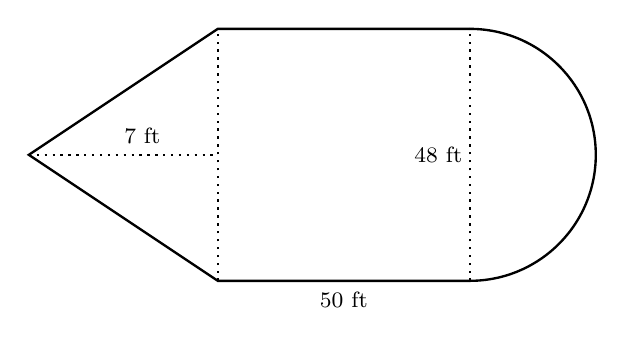
\begin{tikzpicture}[scale=0.8]
	\draw[line width=0.03cm] (4,-2) -- (0,-2) -- (-3,0) -- (0,2) -- (4,2);
	\draw[line width=0.03cm] (4,-2) arc(-90:90:2);
	
	\draw[line width=0.03cm,dotted] (-3,0) -- (0,0);
	\draw[line width=0.03cm,dotted] (0,-2) -- (0,2);
	\draw[line width=0.03cm,dotted] (4,-2) -- (4,2);
	
	\node at (-1.2,0.3) {\footnotesize 7~ft};
	\node at (2,-2.3) {\footnotesize 50~ft};
	\node at (3.5,0) {\footnotesize 48~ft};
	\end{tikzpicture}
	\] 

\sol We can use the symmetry of the diagram to fill it a bit more information:
	\[
	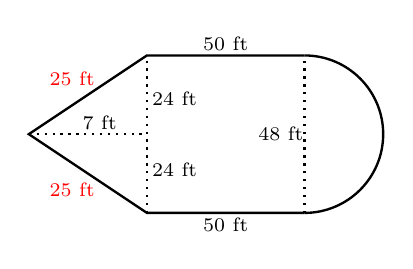
\begin{tikzpicture}[scale=0.5]
	\draw[line width=0.03cm] (4,-2) -- (0,-2) -- (-3,0) -- (0,2) -- (4,2);
	\draw[line width=0.03cm] (4,-2) arc(-90:90:2);
	
	\draw[line width=0.03cm,dotted] (-3,0) -- (0,0);
	\draw[line width=0.03cm,dotted] (0,-2) -- (0,2);
	\draw[line width=0.03cm,dotted] (4,-2) -- (4,2);
	
	\node at (-1.2,0.3) {\scriptsize 7~ft};
	\node at (2,-2.3) {\scriptsize 50~ft};
	\node at (3.4,0) {\scriptsize 48~ft};
	\node at (0.7,0.9) {\scriptsize 24~ft};
	\node at (0.7,-0.9) {\scriptsize 24~ft};
	\node at (2,2.3) {\scriptsize 50~ft};
	\node at (-1.9,1.4) {\scriptsize \color{red} 25~ft};
	\node at (-1.9,-1.4) {\scriptsize \color{red} 25~ft};
	\end{tikzpicture}
	\] 

We need to find the hypotenuse, $c$, of the triangle. We can use the Pythagorean Theorem:
	\[
	c^2= a^2 + b^2= (7 \text{ ft})^2 + (24 \text{ ft})^2= 49 \text{ ft}^2 + 576 \text{ ft}^2= 625 \text{ ft}^2 \Longrightarrow c= \sqrt{625 \text{ ft}^2}= 25 \text{ ft}
	\]
We know that a perimeter of a circle is $C= \pi d$. The perimeter of the half circle is then $\frac{1}{2}C= \frac{1}{2} (\pi d)= \frac{d}{2} \pi= r \pi$. But then the perimeter is\dots
	\[
	P= 50 \text{ ft} + 25 \text{ ft} + 25 \text{ ft} + 50 \text{ ft} + 24\pi \text{ ft}= 150 \text{ ft} + 24\pi \text{ ft} \approx 225.398 \text{ ft}
	\]
The area of the region is\dots
	\[
	\begin{aligned}
	A&= A_{\Delta} + A_{\Box} + \frac{1}{2} A_{\bigcirc} \\[0.3cm]
	&= \frac{1}{2} bh + \ell w + \frac{1}{2} \cdot \pi r^2 \\[0.3cm]
	&= \frac{1}{2} \cdot 48 \text{ ft} \cdot 7 \text{ ft} + 50 \text{ ft} \cdot 48 \text{ ft} + \frac{1}{2} (24 \text{ ft})^2 \pi \\[0.3cm]
	&= 168 \text{ ft}^2 + 2400 \text{ ft}^2 + 288\pi \text{ ft}^2 \\[0.3cm]
	&= (2568 + 288\pi) \text{ ft}^2 \\[0.3cm]
	&\approx 3,\!472.78 \text{ ft}^2
	\end{aligned}
	\] 
Because the cross-sectional areas of the room are all the same, by Cavalieri's Principle, the volume of the room will be $V= Bh$, where $B$ is the area of the `base' and $h$ is the height. Therefore, we have\dots
	\[
	V= Bh= 8 \text{ ft} \cdot (2568 + 288\pi) \text{ ft}^2= 8(2568 + 288\pi) \text{ ft}^3 \approx 27,\!782.24 \text{ ft}^3
	\]



% Question 6
\newpage
\question[10] Explain why $f(x, y)= x^2 - y + 3$ is a function and find the value of $f$ at $(x, y)= (-1, 5)$. \pspace

\sol For each input, $(x, y)$, there is only one possible output---namely, the one obtained by `plugging-in' for $x, y$ and following order of operations. To find, $f(-1, 5)$, we have\dots
	\[
	f(-1, 5)= (-1)^2 - 5 + 3= 1 - 5 + 3= -4 + 3= -1
	\]



% Question 7
\newpage
\question[10] Consider the function $f(x)= 9 - 2x$. 
	\begin{enumerate}[(a)]
	\item Explain why $f(x)$ is a linear function. 
	\item Find the slope and $y$-intercept for $f(x)$. 
	\item Find the $x$-intercept for $f(x)$. 
	\item Find $f(3)$. 
	\item Find an $x$ such that $f(x)= 5$. 
	\end{enumerate} \pspace

\sol  
\begin{enumerate}[(a)]
\item Because $f(x)$ has the form $y= mx + b$ with $m= -2$ and $b= 9$, we know that $f(x)$ is a linear function. \pspace

\item From (a), we can see that the slope is $m= -2$ and the $y$-intercept is $b= 9$, i.e. the point $(0, 9)$. \pspace

\item The $x$-intercept is where the graph of the function crosses the $x$-axis, where $y= 0$. But then this is the $x$-value where $f(x)= 0$:
	\[
	\begin{gathered}
	f(x)= 0 \\
	9 - 2x= 0 \\
	-2x= -9 \\
	x= \frac{9}{2} \\
	x \approx 4.5
	\end{gathered}
	\]
We can verify: $f(4.5)= 9 - 2(4.5)= 9 - 9= 0$. Therefore, the $x$-intercept is $\frac{9}{2} \approx 4.5$, i.e. the point $(4.5, 0)$. \pspace

\item We have\dots
	\[
	f(3)= 9 - 2(3)= 9 - 6= 3
	\] \pspace

\item If $f(x)= 5$, then\dots
	\[
	\begin{gathered}
	f(x)= 5 \\
	9 - 2x= 5 \\
	-2x= -4 \\
	x= 2
	\end{gathered}
	\]
We can check: $f(2)= 9 - 2(2)= 9 - 4= 5$. 
\end{enumerate}
	


% Question 8
\newpage
\question[10] Find the linear function through the points $(-1, 6)$ and $(3, -4)$. Is this linear function increasing or decreasing? Explain. \pspace

\sol Because the function, say $\ell(x)$, is linear, we know that $\ell(x)= mx + b$, for some $m, b$. We know that $m$ is the slope, i.e. $m= \frac{\Delta \ell}{\Delta x}$. But then\dots
	\[
	m= \frac{\Delta \ell}{\Delta x}= \dfrac{6 - (-4)}{-1 - 3}= \dfrac{6 + 4}{-1 - 3}= \dfrac{10}{-4}= -\dfrac{5}{2} \approx -2.5
	\] \pspace
But then, we know that $\ell(x)= -\frac{5}{2}\,x + b= -2.5x + b$. Because the line contains the point $(-1, 6)$, we know that\dots
	\[
	\begin{gathered}
	\ell(x)= -\frac{5}{2}\,x + b \\
	\ell(-1)= -\frac{5}{2} \cdot -1 + b \\
	6= \frac{5}{2} + b \\
	b= \frac{7}{2} \\
	b \approx 3.5
	\end{gathered}
	\] \pspace
Therefore, we know that\dots
	\[
	\ell(x)= -\frac{5}{2}\,x + \frac{7}{2}= -2.5x + 3.5
	\]



% Question 9
\newpage
\question[10] You keep a secret lunchbox under your bed filled with cash. The lunchbox currently contains \$2,500. Each week, you place \$80 into the lunchbox. Let $M(w)$ denote the amount of money in the lunchbox $w$~weeks from now. 
	\begin{enumerate}[(a)]
	\item Explain why $M(w)$ is linear.
	\item Find $M(w)$. 
	\item Use (b) to find how long until the lunchbox has \$10,000. 
	\end{enumerate} \pspace

\sol 
\begin{enumerate}[(a)]
\item We know that a function with a constant rate of change is linear. The only way the amount of money in the lunchbox changes is because of your weekly \$80 deposits into it. But because you place a constant amount in each week, the amount that the lunchbox changes by a constant amount each week. Therefore, the rate of change of $M(t)$ is constant. Therefore, $M(t)$ must be linear. \pspace

\item From (a), we know that $M(t)$ is linear. Therefore, $M(t)= mt + b$ for some $m, b$. Because $m$ is the rate of change and the amount of money in the lunchbox increases by \$80 per week, we know that $m= 80$. But then $M(t)= 80t + b$. \pspace

At the start, i.e. at time $t= 0$, we know that the lunchbox contained \$2,500. But then $\$2500= M(0)= 80(0) + b= 0 + b= b$. Therefore, $b= \$2500$. But then\dots
	\[
	M(t)= 80t + 2500
	\] \pspace

\item We want to know the time, $t_0$, when the lunchbox will contain \$10,000. But at this time, $M(t_0)= \$10000$. But then\dots
	\[
	\begin{gathered}
	M(t_0)= 10000 \\
	80t_0 + 2500= 10000 \\
	80t_0= 7500 \\
	t_0= 93.75
	\end{gathered}
	\]
Therefore, the lunchbox will contain \$10,000 after 94 weeks.\footnote{After 93 weeks, the lunchbox would only contain \$9,940. As you only deposit money weekly, the next time the amount would increase would be the following week---the 94~week---where the amount would be \$9,940 $+$ \$80, which is \$10,020.}
\end{enumerate}



% Question 10
\newpage
\question[10] You and a coworker are responsible for maintaining a portion of a golf course. You can weed the field in 8~hours. When your coworker helps you, you are able to do it in 5~hours. How fast can your coworker weed the field? \pspace

\sol Let $Y$ stand for you and $C$ stand for your coworker. We know that the number of fields a person can weed, $F$, is the rate at which they weed a field, $r$, times the time that they weed, $t$. But then $F= rt$. Let $F_Y, F_C$ be the number of fields you and your coworker weed, respectively, $r_Y$ and $r_C$ denote the rate at which you and your coworker weed fields, respectively, and $t_Y, t_C$ be the time you and your coworker weed fields, respectively. Therefore, we know that\dots
	\[
	\begin{aligned}
	F_Y&= r_Y t_Y \\[0.3cm]
	F_C&= r_C t_C
	\end{aligned}
	\]
We know that you can weed $F_Y= 1$~field every $t_Y= 8$~hours. But then\dots
	\[
	\begin{gathered}
	F_Y= r_Y t_Y \\
	1= 8r_Y \\
	r_Y= \frac{1}{8}
	\end{gathered}
	\]
We know that you and your coworker working together at a rate $r_T$ can weed a field, i.e. $F_T= 1$, in 5~hours. But then $1=F_T= r_T t_T= 5r_T$. We know that the rate working together should be the sum of your individual rates, i.e. $r_T= r_Y + r_C$, and because we know $r_Y= \frac{1}{8}$, we know $r_T= \frac{1}{8} + r_C$. But then\dots
	\[
	\begin{gathered}
	F_T= r_T t_T \\
	1= 5(\frac{1}{8} + r_C) \\
	1= \frac{5}{8} + 5r_C \\
	\frac{3}{8}= 5r_C \\
	r_C= \frac{3}{40} \approx 0.075 \text{ fields/hr}
	\end{gathered}
	\]
But then, we can compute the time it takes your coworker to weed one field:
	\[
	\begin{gathered}
	F_C= r_C t_C \\
	1= \frac{3}{40} t_C \\
	t_C= \frac{40}{3} \approx 13.33 \text{ hours}
	\end{gathered}
	\]
Therefore, it takes your coworker approximately 13.3~hours to weed a field.


\end{questions}
\end{document}